\section{Bivariate Datenanalyse}
Der nächste Abschnitt widmet sich der bivariaten Datenanalyse. Dabei wird nicht mehr nur unsere Y-Variable "Benzinpreis" \, betrachtet, sondern zusammen mit weiteren Einflussgrößen analysiert, um mögliche Zusammenhänge zu erkennen. Ziel der Analyse ist es, Einflussgrößen zu identifizieren und Zusammenhänge offen zu legen, die in einem weiteren Schritt die Prognose von Werten der beeinflussten Größe ermöglichen.\\
Die zu betrachtenden Einflussgrößen sind BIP\_D, EURUSD, Rohölpreis, Stimmung und OPEC und wurden analog zu den Benzinpreisen pro Monat im Zeitraum von April 2010 bis April 2022 stichprobenartig erfasst.\\
Im Folgenden werden diese Merkmale zunächst anhand ihres Skalenniveaus kategorisiert und dann nacheinander auf ihren linearen Zusammenhang mit der Y-Variablen untersucht. Ähnliche Vorgehensweisen in den Analyseverfahren werden aufgrund der Redundanz nur einmal ausführlich erklärt und danach mit Verweis analog wiederholt.\\



\subsection{Einflussgröße I: Bruttoinlandsprodukt}
BIP\_D steht für das \textbf{Bruttoinlandsprodukt} in Deutschland und wird im vorliegenden Datenmaterial in MRD. € erfasst.\\
Es ist ein Indikator für Wohlstand, Wachstum und Leistungsfähigkeit einer Volkswirtschaft und misst die im gesamten Inland entstandene Wirtschaftsleistung innerhalb eines bestimmten Zeitraumes.\footnote{vgl. bwl-lexikon.de} Da jedes Land im weitesten Sinne \textit{irgendwas} produziert, kann das BIP allenfalls bei Null liegen, jedoch nicht negativ werden, und ist damit \textbf{metrisch verhältnisskaliert.} Zur Analyse des Zusammenhangs wird deshalb auf den Korrelationskoeffizienten zurückgegriffen.\\

\subsubsection{Einleitende Analyse}
\begin{figure}[H]
  \centering
  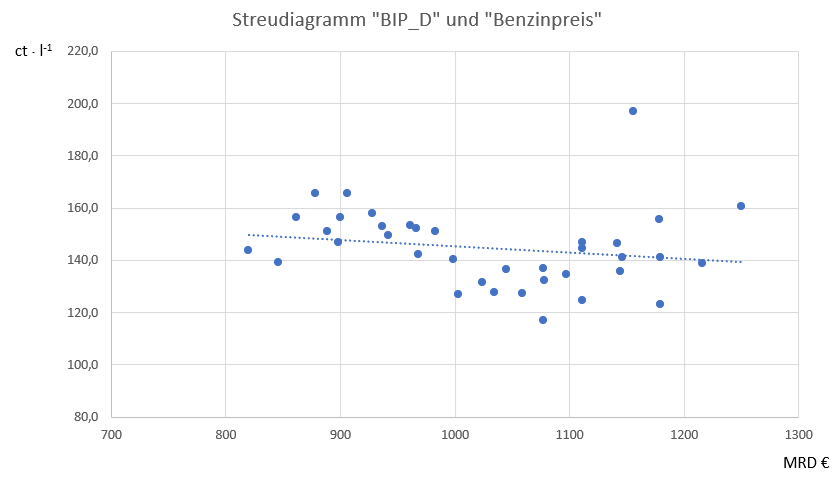
\includegraphics[width = \textwidth]{graphics/streubipbenz.png}
  \caption{Streudiagramm "BIP\_D" \, und "Benzinpreis"}
  \label{fig:streuBipBenz}
\end{figure}

Mithilfe der Trendlinie ist bereits ein schwacher negativer linearer Zusammenhang der beiden Größen vermutbar, da die Punkte recht weit um die Trendlinie herum streuen. Naheliegender scheint ein nicht-linearer Zusammenhang, der durch eine trigonometrische Funktion beschrieben werden kann. Dabei handelt es sich jedoch nur um eine Vermutung und soll hier lediglich als Idee aufgeführt sein.\\

\subsubsection{Mathematische Analyse des linearen Zusammenhangs}
Der Zusammenhang soll nun mithilfe des Korrelationskoeffizienten genauer untersucht werden.\\
Dafür wird in einem ersten Schritt unter Zuhilfenahme einer Arbeitstabelle\footnote{siehe Anhang Arbeitstabelle} die \textbf{Kovarianz} beider Werte (), sowie die individuelle Standardabweichung der Merkmale () ermittelt.

\begin{align}
  s_{xy} = \frac{37}{36} \cdot (\frac{5.499.666,9}{37} - 144,7 \cdot 1.029,7297) = -326,5426 \, \si{\ct\per\liter} \cdot \si{\mrdEuro}
\end{align}

Die Kovarianz gewährt bereits erste Einblicke und weist auf einen negativen linearen Zusammenhang hin. Weitere Aussagen sind an dieser Stelle nicht möglich, da es sich bei der Kovarianz um eine nicht standardisierte Größe handelt.\footnote{vgl. Statistikskript 2022 S. 116}\\

\begin{align}
  s_x^2 &= \frac{37}{36} \cdot (\frac{39.711.148}{37} - 1.029,7297^2) = 13.290,1471 \, [\si{\mrdEuro}]^2\\
  s_x &= \sqrt{13.290,1471 \, [\si{\mrdEuro}]^2} = 115,2829 \,\si{\mrdEuro}
\end{align}

Für die Varianz s\textsubscript{y}\textsuperscript{2} und die Standardabweichung s\textsubscript{y} (des Benzinpreises) können wir die Berechnungen (15) und (16) aus dem vorangegangenen Kapitel übernehmen.\\
Mit diesen Werten können wir nun den Korrelationskoeffizienten ermitteln:

\begin{align}
  r &= \frac{s_{xy}}{s_x \cdot s_y} = \frac{-326,5426 \, \si{\ct\per\liter} \cdot \si{\mrdEuro}}{115,2829 \,\si{\mrdEuro} \cdot 14,926 \, \si{\ct\per\liter}}\\
    &= -0,1898
\end{align}

Der Korrelationskoeffizienten bestätigt die anfängliche Vermutung und zeigt, dass zwischen den untersuchten Merkmalen ein negativer, schwacher linearer Zusammenhang besteht.
Der Benzinpreis fällt also tendentiell höher aus, je niedriger das Bruttoinlandsprodukt.\\

\subsubsection{Test auf lineare Abhängigkeit}
Es besteht jedoch die Möglichkeit, dass der zuvor ermittelte Zusammenhang lediglich zufällig im Rahmen der Stichprobe zustande kam. Aus diesem Grund muss geprüft werden, ob der lineare Zusammenhang auch für die (unbekannte) Grundgesamtheit gültig ist. \\
Dafür wird zunächst die Nullhypothese H\textsubscript{0} formuliert: "Die Merkmale X (BIP\_D) und Y (Benzinpreis) sind linear unabhängig."\\

Um die Gültigkeit der Nullhypothese zu testen, wird eine Testgröße T benötigt, die mithilfe des Korrelationskoeffizienten  berechnet werden kann:

\begin{align}
  T &= \frac{r}{\sqrt{1-r^2}} \cdot \sqrt{n-2}
    &= \frac{-0,1898}{\sqrt{1-(-0,1898)^2}} \cdot \sqrt{37-2}
    &= -1,1435
\end{align}

Im Folgenden wird die Signifikanzwahrscheinlichkeit einer t-verteilten Zufallsvariablen mit df = 37-2 = 35 Freiheitsgraden X\textsubscript{t;35} mithilfe der Excelfunktion T.VERT bestimmt. Etwas trivialer formuliert könnte man sagen: Es wird geprüft, wie hoch die Wahrscheinlichkeit dafür ist, dass eine Zufallsvariable (t-verteilt, mit df - Freiheitsgraden) den in der Stichprobe ermittelten Wert der Testgröße mindestens erreicht. Dafür wird die ermittlete Wahrscheinlichkeit mit dem festgelegten Signifikanzniveau von $\frac{\alpha}{2}$ = 0,025 bzw. 2,5\% verglichen.

\begin{align}
  P(X_{t;35} \leq T) &= 1 - \exceltvert{-1,1435}{35}\\
                      &= 0,86971
\end{align}

Da die ermittelte Signifikanzwahrscheinlichkeit mit 86,971\% weit über dem Signifikanznivea liegt, kann die Nullhypothese nicht abgelehnt werden. Demnach besteht außerhalb der Stichprobe kein signifikanter linearer Zusammenhang zwischen dem Bruttoinlandsprodukt und dem Benzinpreis.



\subsection{Einflussgröße II: Wechselkurs Euro $\rightarrow$ USD}
EURUSD steht für den \textbf{Wechselkurs von EURO in USD}. Zwar wir im vorliegenden Datenmaterial keine eindeutige Aussage über die Einheit getroffen, rein logisch müssten die Werte jedoch in USD $\cdot$ €\textsuperscript{-1} vorliegen. Aufgrund der Erfassung wird zudem von einem durchschnittlichen Wechselkurs für den betrachteten Monat ausgegangen.\\
Der Wechselkurs stellt das Verhältnis der Werte von einer Währungseinheit zu einer anderen dar. Da ein Verhältnis nicht negativ bzw. kleiner 0 werden kann und die Abstände zwischen den Werten gleichmäßig und messbar sind, liegt ein \textbf{metrisch verhältnisskaliertes Merkmal} vor. Die Analyse des Zusammenhangs erfolgt deshalb mithilfe des Korrelationskoeffizienten.

\subsubsection{Einleitende Analyse}
\begin{figure}[H]
  \centering
  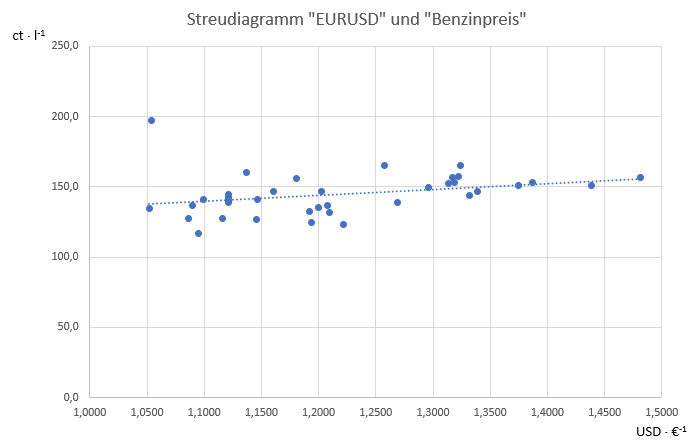
\includegraphics[width = \textwidth]{graphics/streueurusdbenz.png}
  \caption{Streudiagramm "EURUSD" \, und "Benzinpreis"}
  \label{fig:streuEURBenz}
\end{figure}

Anhand des Streudiagramms lässt sich bereits ein positiver linearer Zusammenhang vermuten, der aufgrund der Streuung um die Trendlinie tendentiell schwach bis mittelmäßig ausfallen wird.\\

\subsubsection{Mathematische Analyse des linearen Zusammenhangs}
Wie im Kapitel zuvor, soll nun der Zusammenhang mathematisch analysiert werden.
Dafür werden die Kovarianz\footnote{vgl. Berechnung 18 Kapitel 2.1.2} und - ergänzend zu dem Wert der Standardabweichung für Merkmal Y - die Standardabweichung für Merkmal X\footnote{vgl. Berechnung 19/20 Kapitel 2.1.2} berechnet. Die ermittelten Werte dienen dann der Berechnung des Korrelationskoeffizienten\footnote{vgl. Berechnung 21/22 Kapitel 2.1.2}.

\begin{align}
  s_{xy} &= 0,5084 \, \si{\ct\per\liter} \cdot \si{\usd\per\euro}\\
  s_{x}^2 &= 0,0125 \, [\si{\usd\per\euro}]^2\\
  s_x &= 0,1116 \, \si{\usd\per\euro}\\
  r &= 0,3052
\end{align}

Mit einem Korrelationskoeffizienten von 0,3052 ist von einem mittelmäßigen, positiven linearen Zusammenhang zwischen den Merkmalen X (EURUSD) und Merkmal Y (Benzinpreis) auszugehen. Tendentiell steigt der Benzinpreis also mit steigendem Wechselkurs.

\subsubsection{Test auf lineare Abhängigkeit}
Die Nullhypothese H\textsubscript{0} für den vorliegenden Sachverhalt lautet: "Die Merkmale X (EURUSD) und Y (Benzinpreis) sind linear unabhängig."\\
Für den Test der Signifikanz des Korrelationskoeffizienten, wird nun die Testgröße ermittelt und die Signifikanzwahrscheinlichkeit bestimmt:

\begin{align}
  T &= 1,8957\\
  P(X_{t;35} \geq T) &= 1 - \exceltvert{1,8957}{35}\\
                    &= 0,0331
\end{align}

Die Signifikanzwahrscheinlichkeit liegt damit knapp über dem halbierten Signifikanzniveau von 0,025. Die Nullhypothese kann damit nicht abgelehnt werden; es besteht kein signifikanter linearer Zusammenhang zwischen dem Wechselkurs EURUSD und dem Benzinpreis.



\subsection{Einflussgröße III: Rohölpreis}
Der vorliegende \textbf{Rohölpreis} beschränkt sich auf die Ölsorte Brent. Das ist wenig verwunderlich, denn Brent ist inzwischen die Referenzsorte für den Weltmarkt und damit repräsentativer Indikator für globale Ölpreise.\footnote{vgl. Kimani, o.S.} Sie werden in USD $\cdot$ bbl\textsuperscript{-1} angegeben.\\
Da die Preise für Öl den Benzinpreisen in ihrer Art sehr ähnlich sind, lassen sie sich als \textbf{metrisch verhältnisskalierten Merkmal} definieren; der Korrelationskoeffizient dient auch hier als Instrument zur Analyse des Zusammenhangs. Leider sind keine Aussagen dazu getroffen, ob es sich um einen Durchschnittswert oder konkreten Wert zum Ende des betrachteten Monats handelt. Da der Benzinpreis ebenfalls als durchschnittlicher Preis erfasst wurde, wird der Vollständigkeit halber an dieser Stelle ebenfalls von einem durchschnittlichen Rohölpreis ausgegangen.\\

\subsubsection{Einleitende Analyse}
\begin{figure}[H]
  \centering
  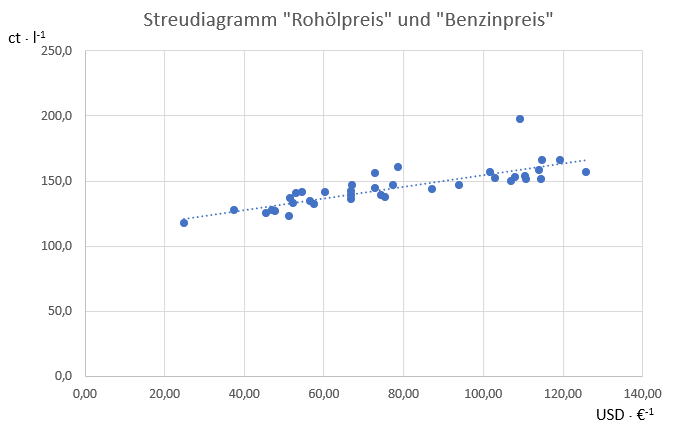
\includegraphics[width = \textwidth]{graphics/streurohbenz.png}
  \caption{Streudiagramm "Rohölpreis" \, und "Benzinpreis"}
  \label{fig:streuRohBenz}
\end{figure}
Im Kontrast zu den vorangegangenen Merkmalen lässt sich hier ein mittelmäßiger bis starker positiver linarer Zusammenhang vermuten. Die Punkte liegen nah bei der eingezeichneten Trendlinie und streuen bis auf wenige Ausnahmen nur schwach um diese herum.\\

\subsubsection{Mathematische Analyse des linearen Zusammenhangs}
Wie bei den Merkmalsanalysen zuvor, soll auch hier die Vermutung mathematisch untersucht werden. Dafür werden wieder Kovarianz und Standardabweichung des neuen Merkmals X (Rohölpreis) ermittelt und aus ihnen sowie den bereits vorhandenen Werten für Merkmal Y (Benzinpreis) der Korrelationskoeffizient berechnet.

\begin{align}
  s_{xy} &= 327,8951 \, \si{\ct\per\liter} \cdot \si{\usd\per\bbl}\\
  s_{x}^2 &= 743,2488 \, [\si{\usd\per\bbl}]^2\\
  s_x &= 27,2626 \, \si{\usd\per\bbl}\\
  r &= 0,8058
\end{align}

Der Korrelationskoeffizient beträgt in diesem Fall 0,806 und weist damit auf einen starken linearen positiven Zusammenhang zwischen den beiden betrachteten Merkmalen hin. Steigt der Preis für Rohöl, wird höchst wahrscheinlich auch der Preis für Benzin steigen.

\subsubsection{Test auf lineare Abhängigkeit}
Im Zuge des Tests auf lineare Abhängigkeit wird folgende Nullhypothese H\textsubscript{0} formuliert: "Die Merkmale X (Rohölpreis) und Y (Benzinpreis) sind linear unabhängig."\\
Für den Test der Signifikanz des Korrelationskoeffizienten wird nun die Testgröße ermittelt und die Signifikanzwahrscheinlichkeit bestimmt:

\begin{align}
  T &= 8,0504\\
  P(X_{t;35} \geq T) &= 1 - \exceltvert{8,0504}{35}\\
                    &= 0,00000...
\end{align}

Die Signifikanzwahrscheinlichkeit fällt so gering aus, dass es aus Gründen der Verständlichkeit anschaulicher erscheint, das Ergebnis der T.VERT-Funktion zu zeigen. Mit 0,99999... fällt dieses erstaunlich hoch aus; die Signifikanzwahrscheinlichkeit liegt damit weit unter dem Signifikanzniveau und führt damit zur Ablehnung der Nullhypothese.\\
Der positive lineare Zusammenhang zwischen Rohölpreis und Benzinpreis ist damit signifikant.



\subsection{Einflussgröße IV: Stimmungsindikator}
Der \textbf{Stimmungsindikator} wird im Rahmen des vorliegenden Materials als Stimmungsindikator am Markt für Rohöl definiert. Stimmungsindikatoren sind - vereinfacht gesagt - Verhältniszahlen, die Aufschluss über Trends, Vermögenswerte und die Wirtschaft aus einer entsprechenden Perspektive geben.\footnote{vgl. bienngoccruise.com} Für den Rohölmarkt wird dieser Indikator mit einem Wert = 1 als neutral, einem Wert < 1 als negativ und einem Wert > 1 als positiv beschrieben.\\
Per se funktionieren Stimmungsindikatoren wie Barometer, wobei sie nie einen Wert unter 0 erreichen, der Wertebereich jedoch nach oben offen bleibt. Dabei ist die Aussagekraft der Werte unterschiedlich und die Bedeutung ihrer Abstände nicht eindeutig bestimmbar. Aus diesem Grund handelt es sich um ein quasi-stetig \textbf{ordinal skaliertes Merkmal}, für die folgende Analyse wird der \textbf{Rangkorrelationskoeffizient} verwendet.\\

\subsubsection{Einleitende Analyse}
\begin{figure}[H]
  \centering
  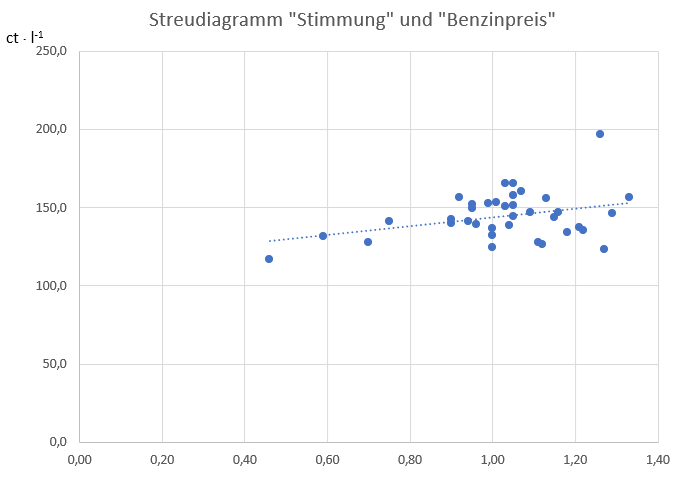
\includegraphics[width = \textwidth]{graphics/streustimbenz.png}
  \caption{Streudiagramm "Stimmung" \, und "Benzinpreis"}
  \label{fig:streuStimBenz}
\end{figure}
Das Streudiagramm lässt bereits einen schwachen positiven linearen Zusammenhang vermuten. Obgleich die Werte zum den niedrigen Stimmungsindikatorwert nahe bei der Trendlinie liegen, streuen sie doch immer extremer, je positiver der Wert wird. Der konkrete Zusammenhang soll im Weiteren wieder mathematisch analysiert werden.

\subsubsection{Mathematische Analyse des monotonen Zusammenhangs}
Aufgrund der unterschiedlichen Skalenniveaus ist die Berechnung von Kovarianz und Korrelationskoeffizienten hier nicht ohne weiteres möglich.\\
Stattdessen werden die Werte der Stimmung und des Benzinpreises mithilfe einer Arbeitstabelle\footnote{siehe Anhang Arbeitstabelle } ihren Werten entsprechend aufsteigend mit Rängen versehen. Die Ränge können nun wie ein metrisches Merkmal behandelt und verrechnet werden.\\
Analog zu den vorherigen Kapiteln wird aus der Summe der Rangprodukte die Kovarianz errechnet, sowie die Standardabweichungen der individuellen Merkmalsränge. Die vorliegenden Werte können dann zur Berechnung des Rangkorrelationskoeffizienten genutzt werden:

\begin{align}
  s_{R(x)R(y)} &= \frac{37}{36} \cdot (\frac{14.082,5}{37} - 19 \cdot 19) = 20,1528\\
  s_{R(x)}^2 &=  \frac{37}{36} \cdot (\frac{17.566,5}{37} - 19^2) = 116,9306 \Rightarrow s_{R(x)} &= 10,8134\\
  s_{R(y)}^2 &=  \frac{37}{36} \cdot (\frac{17.574}{37} - 19^2) = 117,1389 \Rightarrow s_{R(y)} &= 10,8231 \\
  R &= \frac{s_{R(x)R(y)}}{s_{R(x)} \cdot s_{R(y)}} = \frac{20,1528}{10,8134 \cdot 10,8231} = 0,1722
\end{align}

Mit einem Wert von 0,1722 deutet der Rangkorrelationskoeffizient auf einen schwachen positiven monotonen Zusammenhang der gebildeten Rangzahlen hin. Steigt die Rangzahl von X, erhöht sich tendentiell auch die Rangzahl von Y. Berücksichtigt man die Transformation und damit die ursprünglichen Merkmale, bedeutet dies, dass tendentiell der Benzinpreis steigt, wenn die Stimmung am Rohölmarkt steigt bzw. positiver wird.\\
Um eine so allgemeine Aussage tatsächlich treffen zu können, ist es jedoch unabdingbar, das Ergebnis auf Signifikanz zu testen.

\subsubsection{Test auf monotonen Zusammenhang}
Da der vorliegende Rangkorrelationskoeffizient in der angewandten Form dem Korrelationskoeffizienten entspricht, kann auch das gleiche Testverfahren angewandt werden.\\
Die Nullhypothese H\textsubscript{0} lautet: "Die Rangzahlen der Merkmale X (Stimmungsindikator) und Y (Benzinpreis) sind monoton unabhängig."
Dafür wird die Testgröße mithilfe des Rangkorrelationskoeffizienten bestimmt und die Signifikanzwahrscheinlichkeit berechnet.

\begin{align}
  T &= \frac{R}{\sqrt{1-R^2}} \cdot \sqrt{n-2} = \frac{0,1722}{\sqrt{1-0,1722^2}} \cdot \sqrt{37-2} = 1,0342\\
  P(X_{t;35} \geq T) &= 1 - \exceltvert{1,0342}{35}\\
                    &= 0,1541
\end{align}
Die Signifikanzwahrscheinlichkeit von 0,1541 liegt über dem Signifikanzniveau, die Nullhypothese kann nicht abgelehnt werden. Damit liegt kein signifikanter monotoner Zusammenhang vor.



\subsection{Einflussgröße V: Entscheidungsverhalten der OPEC}
\textbf{OPEC} ist eine dauerhafte, zwischenstaatliche, internationale Organisation von 13 erdölexportierenden Mitgliedsstaaten mit Sitz in Wien, deren Ziel die Stabilisierung des Ölpreises auf dem Weltmarkt zum Wohle aller beteiligten ist. Dafür wird die Erdölförderung künstlich verknappt oder gesteigert, um so den Preis zu stabilisieren, zu drücken oder anzuheben.\footnote{vgl. opec.org}\\
Die hier erfassten Daten beziehen sich auf die Verhandlungen der OPEC über konzertierte Aktionen im jeweiligen Zeitraum und ob eine Entscheidung getroffen wurde oder nicht. Die Ausprägungen des Merkmals sind dabei nicht nach Wert sortierbar und können lediglich als gleich oder ungleich unterschieden werden. Damit liegt ein diskretes \textbf{nominal skaliertes Merkmal} vor, für dessen Analyse sich die Maßzahl von Cramèr eignet.

\subsubsection{Einleitende Analyse}
Da für die folgende Analyse mindestens ein nominal skaliertes Merkmal vorliegt, erübrigt sich die Erstellung eines Streudiagramms aus Gründen der Unmöglichkeit.\\
Stattdessen kann eine zweidimensionale Häufigkeitstabelle mit den klassierten Daten des Benzinpreises als Merkmal Y, und den Ausprägungen der OPEC als Merkmal X angefertigt werden.


\begin{figure}[H]
\centering
\small
\begin{tabular}{l|lllll|l}
Merkmal Y   & \textbf{{[}110;130)} & \textbf{{[}130;140)} & \textbf{{[}140;150)} & \textbf{{[}150;160)} & \textbf{{[}160;200)} & SUMME       \\ \hline
Merkmal X   &                      &                      &                      &                      &                      &             \\
\textbf{E}  & 3                    & 4                    & 5                    & 4                    & 2                    & 18          \\
\textbf{kE} & 3                    & 4                    & 5                    & 5                    & 2                    & 19          \\ \hline
SUMME       & 6                    & 8                    & 10                   & 9                    & 4                    & \textbf{37}
\end{tabular}
\caption{zweidimensionale Häufigkeitstabelle der Merkmale OPEC und Benzinpreis}
\end{figure}

Für die Zellen der Häufigkeitstabelle, welche als Grundlage zur Berechnung der Maßzahl von Cramèr genutzt wird, gilt die Bedingung:

\begin{align}
  \frac{h_{j.} \cdot h_{.k}}{n} = e_{jk} \geq 5
\end{align}

Diese Bedigung wird aber nur von einigen wenigen Zellen der Häufigkeitstabelle erfüllt. Um die Aussagekraft der Maßzahl von Cramèr nicht einzuschränken, wird die Häufigkeitstabelle noch einmal verdichtet.

\begin{figure}[H]
  \centering
  \small
\begin{tabular}{l|lll|l}
Merkmal Y   & \textbf{{[}110; 140)} & \textbf{{[}140;150)} & \textbf{{[}150;200)} & SUMME       \\ \hline
Merkmal X   &                       &                      &                      &             \\
\textbf{E}  & 7                     & 5                    & 6                    & 18          \\
\textbf{kE} & 7                     & 5                    & 7                    & 19          \\ \hline
SUMME       & 14                    & 10                   & 13                   & \textbf{37}
\end{tabular}
\caption{verdichtete zweidimensionale Häufigkeitstabelle}
\end{figure}

Um einer ersten Einschätzung über die statistische Abhängigkeit näher zu kommen, werden die bedingten relativen Häufigkeiten wie folgt berechnet:

\begin{align}
  f(y_k|x_j) &= \frac{h_{jk}}{h_{j.}}\\
  f(y_1|x_1) &= \frac{7}{18} = 0,3889
\end{align}

\begin{figure}[H]
\centering
\small
\begin{tabular}{l|lll|l}
Merkmal Y          & \textbf{{[}110; 140)} & \textbf{{[}140;150)} & \textbf{{[}150;200)} & SUMME           \\ \hline
Merkmal X          &                       &                      &                      &                 \\
\textbf{E}         & 0,3889                & 0,2778               & 0,3333               & 1,0000          \\
\textbf{kE}        & 0,3684                & 0,2632               & 0,3684               & 1,0000          \\ \hline
SUMME              & 0,3784                & 0,2703               & 0,3514               & \textbf{1,0000} \\
\textit{DIFFERENZ} & \textit{0,0205}       & \textit{0,0146}      & \textit{-0,0351}     &
\end{tabular}
\caption{zweidimensionale Häufigkeitstabelle mit bedingten relativen Häufigkeiten}
\end{figure}

Die so ermittelten, bedingten relativen Häufigkeiten können spaltenweise verglichen werden.\\
Da sie nicht übereinstimmen, liegt auf alle Fälle eine statistische Abhängigkeit vor. Die maximale Differenz von 0,0351 (Spalte 3) lässt dabei eine sehr schwache Abhängigkeit vermuten. Für eine genauere Aussage genügt jedoch nicht nur die Betrachtung einer Spalte der Häufigkeitstabelle, sondern das Einbeziehen aller Werte oder genauer: die Maßzahl von Cramèr.

\subsubsection{Mathematische Analyse der statistischen Abhängigkeit}
Um die statistische Abhängigkeit zu prüfen, muss zunächst $\chi^2$ berechnet werden.

\begin{align}
  \chi^2 &= n \cdot [(\sum_{j=1}^{m} \sum_{k=1}^{l} \frac{h_{jk}^2}{h_{j.} \cdot h_{.k}})-1]\\
        &= 37 \cdot [(\frac{7^2}{14 \cdot 18} + \frac{5^2}{10 \cdot 18} + ... + \frac{7^2}{13 \cdot 19}) - 1]\\
        &= 37 \cdot (1,0013495 - 1) = 0,0499
\end{align}

Die Maßzahl von Cramèr lässt sich mit dem vorliegenden Wert wie folgt ermitteln:

\begin{align}
  C &= \sqrt{\frac{1}{n} \cdot \frac{\chi^2}{\text{min}((m-1);(l-1))}}\\
    &= \sqrt{\frac{1}{37} \cdot \frac{0,0499}{\text{min}(2-1)(3-1)}}\\
    &= \sqrt{\frac{0,0499}{37}} = 0,0367
\end{align}


Mit einem Wert von 0,0367 bestätigt die Maßzahl von Cramèr damit die eingangs aufgestellte Vermutung: Es besteht eine schwache statistische Abhängigkeit zwischen dem Entscheidungsverhalten der OPEC und den Benzinpreisen. Der Benzinpreis wird vom Entscheidungsverhalten der OPEC kaum beeinflusst.\\


\subsubsection{Test auf statistische Abhängigkeit}
Für den Test auf statistische Abhängigkeit existiert auch für diese Maßzahl ein Verfahren mithilfe einer Testgröße. Im Gegensatz zu den vorangegangenen Berechnungen wird hier $\chi^2$ selbst als Testgröße verwendet und in die Excel-Funktion CHIQU.VERT eingesetzt.

\begin{align}
  df &= (m-1) \cdot (l-1) = (2-1) \cdot (3-1) = 1 \cdot 2 = 2\\
  P({X^2}_2 \geq T) &= 1 - \excelqvert{0,0499}{2}\\
                    &= 0,9753
\end{align}

Der sich daraus ergebende Wert beträgt 0,9753 und führt zur Ablehnung der Nullhypothese. Von einer signifikanten Abhängigkeit zwischen den Merkmalen Y (Benzinpreis) und X (OPEC) kann daher nicht ausgegangen werden.



\subsection{Zwischenergebnis der bivariaten Datenanalyse}
